

\section{Theoretische Grundlagen}
% V-Ansatz Teil 1 – Allgemeiner Rahmen
Das Forschungsfeld der Empfehlungssysteme ist breit und umfasst zahlreiche methodische
Ansätze. In der Praxis haben sich jedoch zwei grundlegende Paradigmen als besonders einflussreich erwiesen:
Das \ac{CBF}, das auf Inhaltsmerkmalen der zu empfehlenden Items basiert und das \ac{CF}, das aus dem kollektiven
Verhalten der Nutzer lernt. Aufgrund der komplementären Stärken und Schwächen dieser Systeme
werden hybride Architekturen in der Nachrichtenbranche als praktikabler Ansatz beschrieben, 
um Relevanz, Diversität und Cold-Start auszubalancieren; 
sie bilden eine solide Grundlage für prototypische Systeme 
(vgl. \cite{wu_personalized_2022,raza_news_2020}).

\subsection{Content-based Filtering}
\label{sec:cbf}
Content-based Filtering (CBF) ist ein Empfehlungsansatz, der auf den Inhaltsmerkmalen von Items basiert, 
um Ähnlichkeiten zwischen ihnen zu bestimmen (vgl. \cite{Lops_CBRS_SOTA_2011}). In der vorliegenden Arbeit 
wird eine spezifische Form des CBF, die Item-zu-Item-Ähnlichkeit, angewendet. Anstatt ein langfristiges Nutzerprofil 
aus der Lesehistorie zu erstellen, wird hierbei ausschließlich der aktuell 
vom Nutzer gelesene Artikel als Referenzpunkt genommen, um thematisch verwandte Inhalte zu finden. Das Nutzerverhalten 
dient in diesem Ansatz also nicht zur Profilbildung, sondern lediglich zur Auswahl des initialen Artikels.

Technisch wird dazu der Inhalt jedes Artikels – bestehend aus Titel und Text – in eine semantische, 
maschinenlesbare Form überführt. Dies geschieht durch den Einsatz von Transformer-basierten Sprachmodellen 
(vgl. \cite{Vaswani_transformer_2017}), die den Text in hochdimensionale numerische Vektoren, sogenannte Embeddings,
transformieren. Jeder Vektor repräsentiert dabei die semantische Position eines Artikels in einem vieldimensionalen Vektorraum. 
Die thematische Ähnlichkeit zwischen zwei Artikeln kann anschließend über gängige Maße wie Kosinus-Ähnlichkeit, 
\ac{MIPS} oder euklidische Distanz quantifiziert werden. Zunächst gilt
\begin{equation}
\label{eq:cosine_similarity}
\cos(u,v) = \frac{u^{T} \cdot v}{\lVert u^{T} \rVert \,\lVert v \rVert}
\end{equation}

Bei L2-normalisierten Vektoren ($\lVert u \rVert = \lVert v \rVert = 1$) sind diese Maße für die Rangbildung äquivalent:
\[
\cos(u,v) = u^{T} \cdot v
\]
In der Praxis wird daher häufig das Skalarprodukt auf normalisierten Vektoren verwendet; 
die resultierenden Ranglisten entsprechen der Kosinus-Ähnlichkeit.

Eine zentrale Herausforderung bei der Implementierung von CBF-Systemen ist die performante Durchführung 
dieser Ähnlichkeitssuche in Echtzeit, insbesondere bei einem großen Korpus von Hunderttausenden Artikeln. 
Eine naive Brute-Force-Suche, bei der jeder Vektor mit jedem anderen verglichen wird, ist für produktive Anwendungen 
zu rechenintensiv und langsam. Daher kommen spezialisierte Vektorindizes für \ac{ANN} zum Einsatz, 
die den Vektorraum partitionieren und komprimieren. Quantisierungsbasierte Ansätze (z.B. Anisotropic Vector Quantization) 
und redundante Repräsentationen mit orthogonalisierten Residuen (z.B. \ac{SOAR}) reduzieren Speicherbedarf und Suchlatenz 
bei kontrolliertem Recall-Verlust (vgl. \cite{avq_2020,soar_2023}).

\subsection{Collaborative Filtering}
\label{sec:cf}

Im Gegensatz zum Content-Based Filtering, das auf den Inhaltsmerkmalen von Items basiert, 
nutzt das Collaborative Filtering (CF) das kollektive Verhalten und die Interaktionsmuster 
aller Nutzer, um Präferenzen zu modellieren. Der Grundgedanke ist, dass Nutzer, die in der 
Vergangenheit ähnliche Vorlieben zeigten, auch in Zukunft ähnliche Interessen haben werden. 
Eine besondere Herausforderung in Domänen wie Nachrichtenportalen besteht darin, dass die 
Interaktionen typischerweise als implizites Feedback vorliegen – beispielsweise als Klicks 
oder Lesezeit – und nicht als explizite Bewertungen wie eine Sterne-Vergabe. Dies erfordert 
spezielle mathematische Verfahren, um aus dem reinen Vorhandensein einer Interaktion eine 
Präferenz abzuleiten.

Ein etablierter und leistungsstarker Ansatz zur Modellierung impliziter Daten ist die 
gewichtete Matrixfaktorisierung (vgl. \cite{hu_collaborative_2008}). Sie zielt 
darauf ab, die User-Item-Interaktionsmatrix in zwei niedrigdimensionale Matrizen zu 
zerlegen, die latente, also verborgene, Merkmale von Nutzern und Items repräsentieren. 
Das zugrundeliegende Optimierungsproblem wird durch die folgende Formel beschrieben:
\begin{equation}
\label{eq:cf}
\min_{\{x_u\},\{y_i\}} \sum_{u,i} c_{ui}\,\bigl(p_{ui} - x_u^\top y_i\bigr)^2 \;+\; \lambda \Bigl(\sum_u \left\lVert x_u\right\rVert^2 + \sum_i \left\lVert y_i\right\rVert^2\Bigr)
\end{equation}
Diese Formel minimiert den Fehler zwischen den Vorhersagen und den tatsächlichen 
Interaktionen, gewichtet nach der Vertrauenswürdigkeit (Konfidenz) jeder Beobachtung.

\begin{itemize}
    \item $x_u$ und $y_i$: Dies sind die latenten Vektoren, die die verborgenen Präferenzen 
    eines Nutzers $u$ bzw. die Eigenschaften eines Items $i$ repräsentieren. Das Ziel des 
    Modells ist es, diese Vektoren zu lernen.
    \item $x_u^\top y_i$: Das Skalarprodukt der beiden Vektoren. Es dient als Vorhersage, 
    wie wahrscheinlich eine Interaktion zwischen Nutzer $u$ und Item $i$ ist.
    \item $p_{ui}$: Eine binäre Präferenzvariable, die angibt, ob eine Interaktion 
    zwischen Nutzer $u$ und Item $i$ beobachtet wurde ($p_{ui}=1$) oder nicht ($p_{ui}=0$).
    \item $c_{ui}$: Der Konfidenz-Term, der angibt, wie viel Vertrauen in die Beobachtung 
    $p_{ui}$ gelegt wird. Er wird oft als $c_{ui}=1+\alpha r_{ui}$ berechnet, wobei $r_{ui}$ 
    die Häufigkeit der Interaktion (z.B. Anzahl der Klicks) und $\alpha$ ein 
    Skalierungsparameter ist. Dies ermöglicht es dem Modell, wiederholten Interaktionen 
    eine höhere Bedeutung beizumessen.
    \item $\lambda$: Ein Regularisierungsparameter, der verhindert, dass die Werte in den 
    latenten Vektoren zu groß werden (Overfitting) und somit die Generalisierungsfähigkeit 
    des Modells verbessert.
\end{itemize}

Ein modernerer Ansatz, das Neural Collaborative Filtering (NCF), erweitert dieses 
Prinzip, indem es das lineare Skalarprodukt ($x_u^\top y_i$) durch ein nichtlineares 
neuronales Netz, ein \ac{MLP}, ersetzt (vgl. \cite{he_neural_2017}). Siehe Abbildung~\ref{fig:ncf_architektur}.
Dadurch kann das Modell komplexere und subtilere Zusammenhänge in den 
Nutzer-Item-Interaktionen erfassen. NCF-Modelle werden typischerweise mit den 
beobachteten positiven Interaktionen und einer Auswahl an zufällig gezogenen 
negativen Beispielen (Negative Sampling) oder den gesamten negativen Artikeln trainiert, 
was für die Modellqualität entscheidend ist.
\begin{figure}[H]
    \centering
    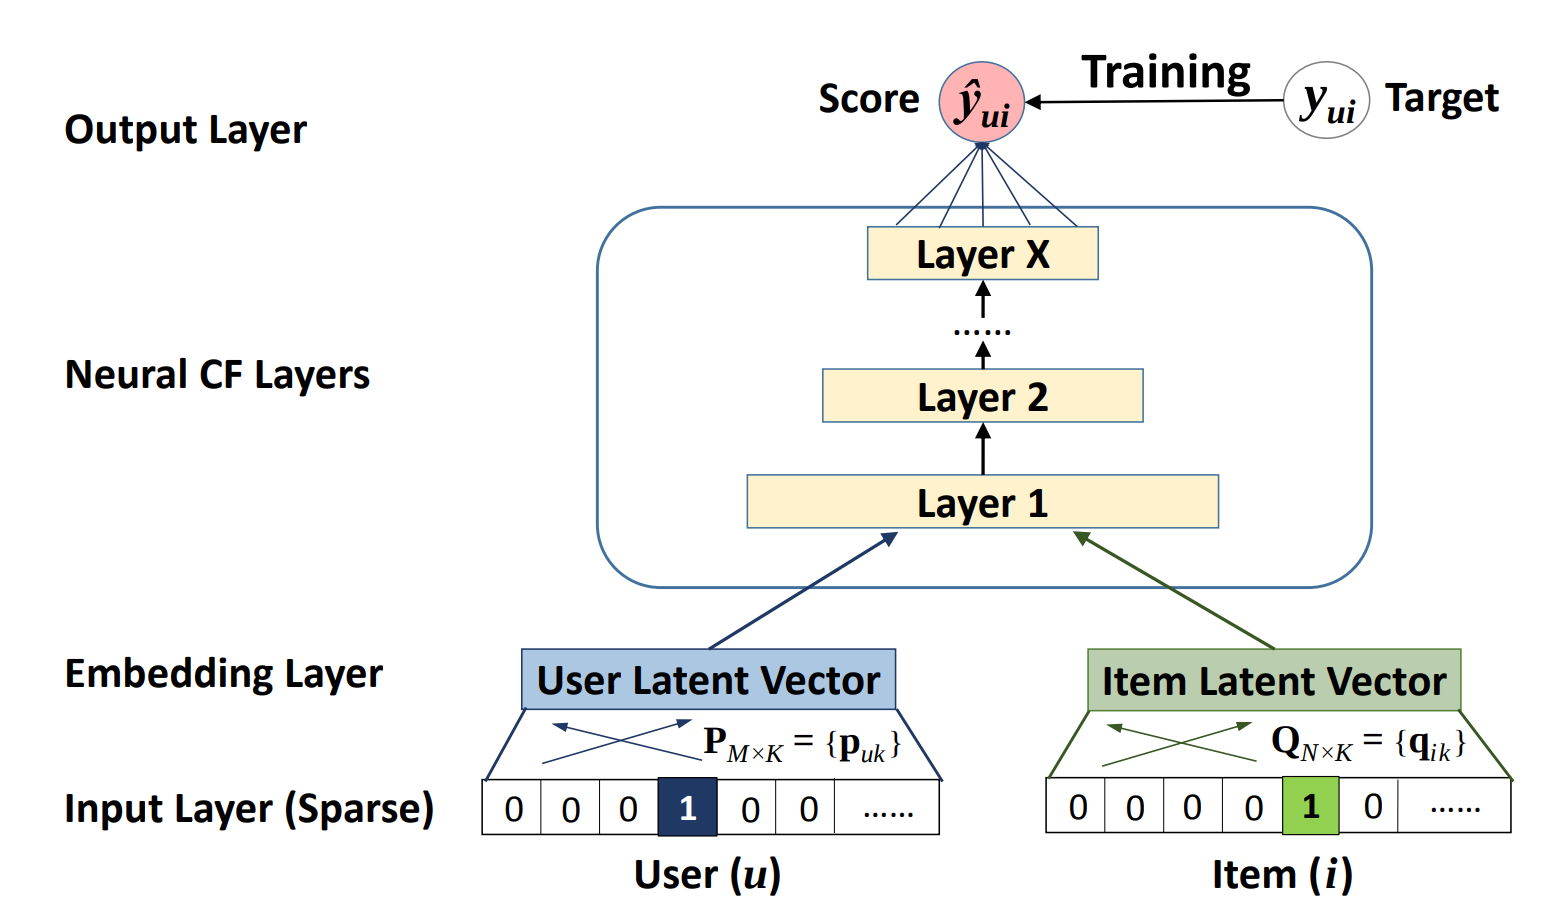
\includegraphics[width=0.6\textwidth]{content/figures/png/img_ncf_diagram.png}
    \caption{Schematische Darstellung der Architektur eines 
    Neural-Collaborative-Filtering-Modells (\Cite{he_neural_2017}).}
    \label{fig:ncf_architektur}
\end{figure}

Trotz ihrer Leistungsfähigkeit weisen CF-Methoden zwei systematische Schwächen auf. 
Erstens leiden sie unter dem Item-Cold-Start-Problem, da sie für neue Artikel ohne 
Interaktionshistorie keine Empfehlungen generieren können. Zweitens neigen sie zu 
einem Popularity Bias, bei dem bereits sehr populäre Artikel überproportional oft 
empfohlen werden, was die Vielfalt und Personalisierung einschränkt 
(vgl. \cite{Abdollahpouri_Popularity_Bias_2019}). Um diese Nachteile zu mitigieren, 
wird der CF-Ansatz in dieser Arbeit mit einem Content-Based-Ansatz kombiniert.

\subsection{Hybrid Filtering}
\label{sec:hybrid}
Da weder \ac{CBF} noch \ac{CF} in isolierter Form alle Anforderungen in der Nachrichtendomäne abdecken, 
gelten hybride Architekturen als praxiserprobter und in der Literatur breit beschriebener Entwurfsansatz. 
Das Ziel ist es, die komplementären Stärken der Ansätze zu kombinieren und deren typische Schwächen 
wie das Item-Cold-Start-Problem oder den Popularity Bias abzumildern 
(vgl. \cite{burke_hybrid_2002,wu_personalized_2022,raza_news_2020}).

Die Fachliteratur unterscheidet eine Vielzahl von Hybridisierungsstrategien. Hierzu zählen unter anderem 
die gewichtete Kombination von Modell-Scores (weighted), eine fallweise Umschaltung zwischen Modellen 
(switching) sowie die Nutzung von Modellergebnissen als Eingangsmerkmale für nachfolgende Modelle 
(feature/meta-level) (vgl. \cite{burke_hybrid_2002}). 
Die vorliegende Arbeit implementiert eine gewichtete Hybridisierung, bei der die Scores der 
\ac{CBF}- und \ac{CF}-Komponente zu einer finalen Empfehlungsliste zusammengeführt werden.

Dieser Ansatz grenzt sich von komplexeren, mehrstufigen Architekturen ab. Bei kaskadierenden 
Systemen (cascade) oder Re-Ranking-Verfahren wird beispielsweise zunächst eine breite Kandidatenliste 
durch ein schnelles Retrieval-Modell erzeugt und diese anschließend in einem zweiten Schritt durch 
ein präziseres, oft aufwendigeres Modell umsortiert. Solche Re-Ranking-Modelle können explizit auf 
weitere Kriterien wie Diversität optimieren, etwa durch die Anwendung von Algorithmen wie 
Maximal Marginal Relevance (MMR) (vgl. \cite{Carbonell_mmr_1998}). Für diese Arbeit wurde bewusst 
eine einstufige, gewichtete Kombination als interpretierbare und robuste Baseline gewählt, deren 
Optimierung im Zentrum der Untersuchung steht.

\subsection{Serendipität}
\label{sec:serendipitaet}
\ac{ES} verfolgen das Ziel, den Nutzern sowohl thematisch ähnliche als auch neuartige und 
unerwartete Inhalte zu präsentieren. Serendipität im allgemeinen Sinne beschreibt das Phänomen, 
zufällige und unerwartete Entdeckungen zu machen, die sich als vorteilhaft erweisen. Im Kontext von \ac{ES} 
lassen sich aus der Literaturübersicht von \cite{Kotkov_Serendipity_2016} drei grundlegende Kriterien ableiten, 
die erfüllt sein müssen, damit eine Empfehlung als serendipitös gilt. Erstens muss das empfohlene Item für den Nutzer 
\textit{relevant} sein, da es sonst als wertlose und irrelevante Ablenkung wahrgenommen würde. Zweitens ist die 
\textit{Neuheit} des Items entscheidend: Der Nutzer darf es zuvor weder gesehen noch davon gehört haben. 
Drittens muss die Empfehlung \textit{unerwartet} sein, indem sie signifikant von den bisherigen Präferenzen des 
Nutzers abweicht. Die Kombination dieser Kriterien stellt sicher, dass eine Empfehlung nicht nur passend, 
sondern auch überraschend und bereichernd ist.

\subsection{Qualitätsdimensionen und Erfolgsmetriken}
Um \ac{ES} miteinander vergleichen zu können, braucht es Metriken, welche die Performace unterschiedlicher
Systeme abbilden können. 

\begin{equation}
\label{eq:dcg}
DCG@K=\sum_{i=1}^{k}\frac{rel_{i}}{\log_2(i+1)}
\end{equation}

\label{sec:idcg}

\begin{equation}
\label{eq:ndcg}
NDCG@K=\frac{DCG@K}{IDCG@K}=\frac{\sum_{i=1}^{k}\frac{rel_{i}}{\log_2(i+1)}}{\sum_{i=1}^{k}\frac{rel_{i}}{\log_2(i+1)}}
\end{equation}

\subsection{Multikriterielle Systeme und Trade-offs}
% Relevanz vs. Vielfalt
% Pareto-Front (nur Konzepte)

% Fußnote: Optional GPT-Prompt-Zitation bei Bedarf
% \footnote{Einige Abschnitte wurden durch KI-gestützte Schreibunterstützung (ChatGPT) vorformuliert und redaktionell überarbeitet.}
